\section{Design and Implementation\label{design}}

\begin{figure}
\center
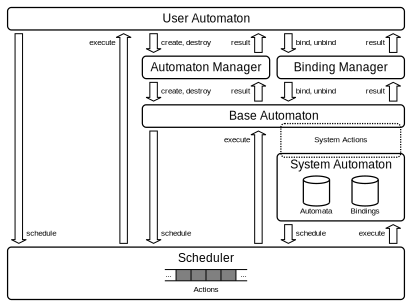
\includegraphics[width=\columnwidth]{architecture}
\caption{Framework architecture.}
\label{framework_architecture}
\end{figure}

The ioa++ framework is a C++ implementation of the component model described in Section~\ref{component_model} (including services for executing local actions and facilities for manipulating the set of automata and bindings), for POSIX environments .
The architecture of the ioa++ framework is depicted in Figure~\ref{framework_architecture}.

Conceptually, state variables belong to the system automaton.
However, the state they encode is shared and is used in the execution of every action.
For a system $S=(A,B)$ consisting of a set of automata $A$ and a set of bindings $B$,
a \emph{scheduler} uses $A$ to ensure that only actions belonging to automata that exist are selected and uses $B$ to ensure that the appropriate set of input actions receive the value produced when an output action is executed.
Thus, the set of actions implied by any action is the union of the set defined in Section~\ref{component_structure} and the system automaton.
The opportunities for concurrent execution discussed in Section~\ref{component_structure} hinge on the fact that \emph{only} actions that modify $A$ and $B$ must be serialized.
The scheduler is responsible for selecting and executing local actions subject to the I/O automata model and the concurrency constraints described in Section~\ref{component_model}.

All user automata inherit from a common base class (indicated by the Base Automaton layer shown in Figure~\ref{framework_architecture}) that provides facilities for asynchronously creating and destroying child automata and bindings.
The Base Automaton layer provides statically composed system actions that are used to communicate with the system automaton.
In most situations, the services provided by the Base Automaton layer are too low-level to be used directly by a user automaton.
Instead, an Automaton Manager provides a common higher-level interface for asynchronously managing a single child automaton using the services of the Base Automaton layer.
Similarly, a Binding Manager presents a high-level interface for asynchronously managing a single binding.

\subsection{Scheduler\label{scheduling}}

The scheduler is responsible for both selecting and executing local actions.
These two activities are decomposed into a \emph{dispatcher} that executes actions and a \emph{controller} that selects the next action.

The dispatcher enforces the execution and concurrency constraints of Section~\ref{component_model}.
Input actions are executed with corresponding output actions, according to the current set of bindings.
The dispatcher allows actions to be executed concurrently by (1)~requiring that the sets of automata implied by each action are disjoint and (2)~serializing all updates to the set of automata and bindings.

Since concurrent access to the dispatcher is allowed, the dispatcher implementation the dispatcher must be thread-safe.
Our implementation of the dispatcher uses a two-level locking scheme to enforce the concurrent execution constraints.
Any action that modifies the set of automata and bindings must first acquire a write lock to prevent concurrent access.
All other actions acquire a read lock to implement single-writer/multiple-reader semantics.
The second phase of executing a non-modifying action involves acquiring locks for the set of automata implied by an action.
The locks are acquired in a fixed order to prevent deadlock~\cite{havender1968avoiding}.
Once the locks are acquired, the precondition is evaluated, the local action and all bound input actions are executed, and the locks are released.

The controller encodes a \emph{policy} that selects the next local action.
For the framework to be a valid implementation of the I/O automata model, the controller used by the scheduler must be \emph{fair} as defined in Section~\ref{component_model}.
The run-time system can be initialized with different controllers to achieve different performance objectives.
To leverage the power of different operating system mechanisms without exposing users to their complexities directly, the ioa++ framework is designed so that all native concurrency and synchronization mechanisms (e.g., threads and mutexes) are encapsulated within the dispatcher and controller.
For example, a controller can be written to use multiple threads of execution to exploit fully the concurrency inherently available in a system of automata,
while still providing concurrency semantics in a manner consistent with the I/O automata component model.

\paragraph*{Explicit dynamic scheduling}
The I/O automata model assumes that the scheduler knows about every local action in the system.
There are two approaches for achieving this in practice.
In the first approach, automata declare \emph{statically} all of their actions to the scheduler.
The controller then has the responsibility of cycling through the actions according to some fair policy.
Since the scheduler has no knowledge about which actions are \emph{enabled} or \emph{disabled} (have a precondition that is true or false respectively), this approach reduces to naively trying each action.

A more focused approach, which is the default approach used in our framework implementation, is to allow automata to declare \emph{dynamically} the actions they would like the scheduler to consider.
%The act of declaring an action to the scheduler is called \emph{scheduling}.
The controller then has the responsibility of processing the set of requested actions according to some fair policy.
Observe that executing an action potentially changes the state of the automaton and causes the set of enabled actions to change.
Consequently, an automaton is given the opportunity to declare actions to the scheduler (i.e., to \emph{schedule} them) after one of its actions is executed.
Since the state variables (and therefore preconditions) of all automata are independent, each automaton is responsible for scheduling its own actions.
For bootstrapping, each automaton is allowed to schedule actions when it is created.

In this approach, scheduling disabled actions is unnecessary.
In order for a scheduled disabled action $a$ to become enabled, the automaton associated with the action must change state by executing another enabled action $b$ sometime after $a$ is scheduled.
Consequently, the scheduling of the disabled action $a$ can be deferred until the execution of some other action.
Notice that refraining from scheduling disabled actions does not affect the fairness of the scheduler since they cannot cause a state change when selected.
This result leads to a guarded programming idiom where the precondition of each action is checked before it is added to the schedule.

However, an automaton must still ensure that the scheduler will \emph{consider} all actions that are currently enabled.
A simple technique for accomplishing this is to schedule all enabled actions.
More efficient schemes are possible if one considers how an action might enable other actions and which actions have already been scheduled.
However, this must be done carefully, since not considering an enabled action would violate the fairness of the controller.
% since it will never select an action that may cause a state change.
% Not scheduling an (enabled) action is a common mistake.

\paragraph*{Binding predicates and scheduling}
%% This assumption is not implicit because we state that the preconditions are independent.
The preceding discussion on scheduling assumed that an action in one automaton cannot affect preconditions in another automaton.
This is not entirely correct when one considers the system automaton and binding predicates.
For example, imagine an automaton with a single output action whose only precondition is that it must be bound and assume that the automaton only schedules the action when enabled.
When the automaton is created, its only action is disabled.
Consequently, it will not schedule its action and therefore will not be executed.
Suppose that some time after the automaton is created, another automaton successfully binds to the output action.
The bind action changes the precondition but the automaton will never be executed since it has no way of scheduling the output action.
While this example may seem contrived, it is representative of situations where an automaton is waiting for one or more of its outputs to be bound: a situation that occurs quite often in practice.
To remedy this, our framework takes advantage of the fair scheduling criteria of the I/O automata model and schedules an output action after each successful bind or unbind.

\paragraph*{Actions of no-longer-existing automata}
Every action in the set of actions considered by the controller is scheduled by its associated automaton.
Since automata can be destroyed, an action in the set owned by the controller might belong to an automaton that no longer exists.
Our solution is to check if the automaton exists before executing an action.
This check is performed by the dispatcher and avoids the overhead associated with synchronizing the set of actions with the set of automata every time an automaton is destroyed.
Our solution assigns each automaton a unique identifier assuming that the set of automata in the system turn over less frequently overall than the set of actions that have been scheduled.

\paragraph*{Delayed actions}
Scheduling activities for a future time is a useful feature for many systems because it allows the system to sleep between activities. For example, the framework should support the development of automata that act as timers and alarms.
Conceptually, an action is held until the time associated with it, at which point it is added to the set of actions being considered by the scheduler.
Actions scheduled in the past or present are released immediately to the scheduler.
When the same action is scheduled at two different times, the earliest time is used.
% Things I didn't say:  No canceling.

\paragraph*{File descriptor events}
File descriptors are used to communicate with the outside world in a POSIX environment.
Observe that there is no concept of blocking in the I/O automata model and introducing blocking I/O operations into action effects may adversely affect the asynchronous and concurrent nature of I/O automata.
Thus, we require techniques that allow a program (1) to wait until a file descriptor is asynchronously ready for I/O and (2) to perform non-blocking I/O operations.
This implies the use of either the Proactor or Reactor pattern~\cite{schmidt2000pattern}.
The ioa++ framework uses the Reactor pattern since (1) it is simpler and (2) many operating systems have non-blocking I/O and some kind of synchronous I/O (de)multiplexing, whereas asynchronous I/O is less widespread.

Our use of the Reactor pattern causes an action to be scheduled when a file descriptor is ready for reading or writing.
A user automaton creates a file descriptor and configures it for non-blocking I/O.
The automaton then tells the scheduler to release an action (typically an internal action) whenever the automaton becomes ready for reading (or writing).
Subsequent requests made using the same file descriptor and event (ready for reading, ready for writing) are ignored.
Once the file descriptor is ready, the action is released for consideration by the controller.
The scheduler also provides a special function for closing file descriptors that purges them from the reactor.

\paragraph*{Basic and multi-threaded schedulers}
The ioa++ framework distribution provides both a basic scheduler that is single-threaded and uses a single queue of actions that is processed using first-in/first-out semantics, and a multi-threaded scheduler with a configurable number of threads that we use in the performance evaluation described in Section~\ref{evaluation}.
Scheduling is idempotent to prevent unbounded growth of the queue, and both scheduler implementations use the Reactor pattern to implement delayed actions and file descriptor events.

\subsection{System Actions\label{system_action_section}}

Our approach to system actions follows the model introduced in Section~\ref{dynamics}.
All automata are statically composed with a system automaton via system actions for dynamically creating child automata, binding external actions, unbinding external actions, and destroying child automata.
The system automaton implements a request-response protocol where an automaton requests a system action and the system automaton processes the request and responds with an indication of either success or failure.
Associated with each request is a \emph{subject} which is the automaton's local name for an automaton or binding.
Subjects allow an automaton to have multiple requests outstanding at once.

Automata use a simple protocol for creating and destroying child automata.
Each child automaton is represented by a unique subject which is in one or two of five states: CreateSend, CreateRecv, CreateDone, DestroySend, and DestroyRecv.
Subjects start in the CreateSend state which indicates that the request for this subject is waiting to be sent to the system automaton.
Once the request has been sent, the subject transitions to the CreateRecv state and waits for a response from the system automaton.
Once the system automaton sends the response, the subject transitions to the CreateDone state.
When the user automaton requests that the child automaton be destroyed, the subject is either (1) added to the DestroySend state if the subject is in CreateRecv or CreateDone or (2) removed from all states if the subject is in CreateSend.
A subject appearing in both CreateDone and DestroySend transitions to the DestroyRecv state when the automaton makes the request to destroy it.
The system automaton can process system actions in any order.
This protocol ensures that an automaton doesn't request that a child automaton be destroyed until it receives confirmation that it was created.
The subject is forgotten when the system automaton responds with the result of the destroy action.

The protocol for binding is similar but addresses the possibility that a binding can be dissolved at any point due to the asynchronous destruction of automata.
We define analogous states for the binding state machine: BindSend, BindRecv, BindDone, UnbindSend, and UnbindRecv.
A binding subject can be in either BindRecv, BindDone, UnbindSend, or UnbindRecv when it receives a result from the system automaton indicating that the binding was dissolved.

\paragraph*{Automaton and Binding managers}
The protocol used by automata to asynchronously manage child automata and bindings is suitable for simple constellations but becomes unwieldy when creating more complicated ones.
Automaton Managers and Binding Managers provide individualized facades to the system action state machines.
Creating an Automaton Manager initiates the creation of a new child automaton and invoking a destroy method initiates the destruction of a child automaton.
Automaton Managers can be monitored using the Observer~\cite{gamma1995design} pattern to determine when and how the creation/destruction process succeeds.
Binding Managers are similar except they do not begin the process of binding until the automata providing the output action and input action have been created: thus, Binding Managers observe Automaton Managers.

\ifjournal
\paragraph*{Generators}
A \emph{generator} is a single-use factory for creating an instance of an automaton.
Generators are used to produce new automata as part of the create system action and are visible as arguments in the various layers of the framework.
\fi
